\begin{figure}
    \centering
    
    \caption*{\textbf{AMZN}}
    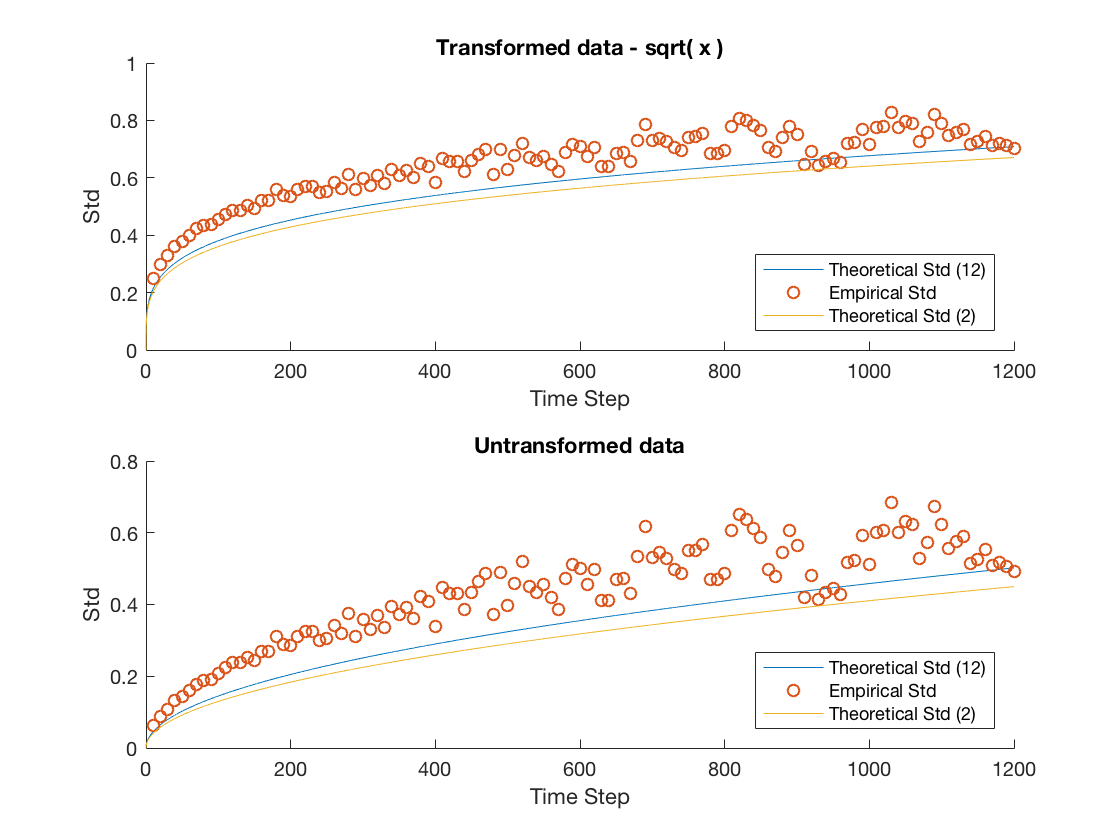
\includegraphics[width=\textwidth]{N_State_Plots/AMZN_N_State.png}
    
    \caption{\label{fig:AMZN_data} We consider the N-state model for AMZN discussed previously in the paper. While there is a slight improvement against the original fit, the model still struggles to perfectly predict the variability in the mid price changes of our data. Comparing the mean residuals, the 2-state model discussed before has mean residual $0.0208$ while our 12-state Markov chain brings that down to $0.0125$. Considering an even larger Markov chain with 24-states we are only able to obtain a meager improvement to $0.0123$, suggesting that there is some underlying variance in the mid price process not captured by our model.}
    
\end{figure}